\chapter{Un regard évolutif}
{\hypersetup{linkcolor=GREYDARK}\minitoc}
\label{chap:evolution}

\section{Évolution de l’expression des gènes}
\label{sec:evolution-gene}

Une grande partie de la variation observée entre individus en termes de niveaux d'expression génétique est héritable et a souvent une base génétique \citep{emilsson_genetics_2008,aguet_genetic_2017}. L’expression des gènes peut donc être considérée comme un phénotype moléculaire intermédiaire, qui est fortement lié aux phénotypes morphologiques et physiologiques.

\subsection{Un modèle d’évolution quasi-neutre pour l’expression des gènes}
\label{subsec:modele-neutre}

Afin d’interpréter les résultats des études comparatives de l’expression des gènes entre espèces et d’en inférer des scénarios évolutifs, il est important de déterminer si les différences observées sont le résultat de la sélection naturelle ou de processus stochastiques. La sélection naturelle joue un rôle majeur en filtrant les organismes les mieux adaptés à leur environnement. Cependant la sélection naturelle agit seulement à l’échelle des phénotypes alors que la variation est générée à l’échelle du génotype. Toutes les mutations n'entraînent pas des modifications phénotypiques, et on peut donc s’attendre à ce que la proportion des changements sélectifs décroisse graduellement à mesure que l’on s’éloigne du phénotype. Kimura a ainsi proposé que la grande majorité des différences observées entre les génomes des espèces n’affectent pas ou très peu les phénotypes des organismes, elles n’ont pas d’impact sur la valeur sélective des individus et sont donc neutres \citep{kimura_neutral_1983}. D’après un modèle quasi-neutre d’évolution moléculaire initié par Kimura et complété par Ohta, la majorité des mutations seraient soit délétères et éliminées par la sélection naturelle dite alors purifiante, soit faiblement délétères et ségrègeraient alors dans les génomes par dérive génétique \citep{ohta_synonymous_1995}. La probabilité de fixation d’une mutation faiblement délétère dépend de son impact sur la survie et la reproduction d’un individu mesuré par un coefficient de sélection et de la taille efficace de la population \citep{charlesworth_effective_2009}. Une population avec un plus grand nombre d’individus reproducteurs est en mesure de filtrer plus efficacement les mutations ayant un faible coefficient de sélection \citep{ohta_slightly_1973}. Les mutations arriveraient alors à fixation soit par dérive génétique, soit beaucoup plus rarement par sélection positive lorsque la mutation présente un avantage suffisant pour l’individu. La conséquence de ce modèle implique que la majorité des différences entre les espèces sont déterminées par des processus non adaptatifs que sont la mutation et la dérive génétique. \\

Est-il possible d’utiliser ce modèle quasi-neutre d’évolution moléculaire, développé pour décrire la divergence des séquences, pour proposer un modèle nul de l‘évolution de l’expression des gènes ? On s'attendrait alors à ce que le taux d’évolution du niveau d’expression soit fortement dépendant du taux de mutation, de la taille de la population et de la contrainte agissant sur le niveau d’expression du gène. Dans le cas d’une évolution dominée par des processus non adaptatifs, les différences entre les espèces devraient s’accumuler de manière approximativement linéaire avec le temps de divergence. De plus, la variation de l’expression d’un gène entre espèces devrait être liée à la variation de l’expression de ce gène dans une population. Les écarts à ces prédictions de l’hypothèse nulle pourraient alors permettre de détecter des changements adaptatifs de l’expression des gènes.\\

Kaitovich et ses collaborateurs ont tenté de tester ces prédictions pour l’évolution de l’expression en décrivant les différences dans les transcriptomes de plusieurs espèces proches de primates \citep{khaitovich_neutral_2004}. Premièrement, ils ont observé que l’accumulation de différences du niveau d’expression d’environ 12 000 gènes dans le cortex préfrontal est effectivement linéaire avec le temps de divergence entre les paires d’espèces (Figure \ref{fig:Fig24}.A). Autrement dit, les variations du niveau d’expression des gènes reflètent les relations phylogénétiques selon un principe d’horloge moléculaire, ce qui confirme la première prédiction d’un modèle quasi-neutre. Ils ont ensuite comparé la divergence inter-espèces du niveau d’expression de près de 3 000 gènes actifs ayant le plus et le moins de variations entre différents individus humains (Figure \ref{fig:Fig24}.B). Les gènes ayant le plus de variations chez l’humain accumulent des différences entre espèces significativement plus rapidement que les autres, ce qui semble cohérent avec la seconde prédiction du modèle. De plus, la différence du niveau d’expression des gènes entre individus chez l’humain est corrélée positivement à la divergence entre espèces de primates. Cette relation entre la variation de l’expression des gènes entre individus et entre espèces est comparable à celle observée pour des séquences d’ADN. Ces observations permettent de poser les bases d’un modèle d’évolution quasi-neutre pour l’évolution de l’expression des gènes similaires à celui de l’évolution des séquences d’ADN, où les différences fixées par dérive génétique sont principalement neutres.

\begin{figure}[h]
    \centering
    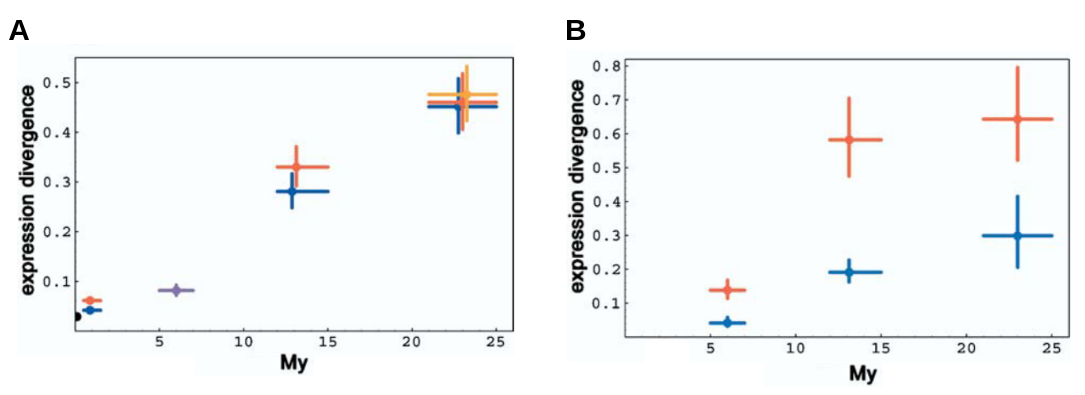
\includegraphics[width=1\textwidth, page=1] {figures/introduction/fig24.png}
    \caption[Divergence des niveaux d'expression des gènes chez les primates.]{
    \textbf{Divergence des niveaux d'expression des gènes chez les primates.}
    \textbf{A.} Différences moyennes d'expression des gènes dans le cerveau au sein et entre primates selon le temps de divergence. Couleurs : rouge, comparaisons entre et avec les humains ; bleu, comparaisons entre et avec les chimpanzés ; violet, comparaisons entre humains et chimpanzés ; orange, comparaisons entre orang-outan et macaque rhésus ; noir, comparaisons entre duplicats expérimentaux.  Les barres d'erreur verticales pour l'expression indiquent les intervalles de confiance à 95\% calculés par 10 000 bootstraps. Les temps de divergence sont selon Glazko et Nei (2003). \textbf{B.} Différences moyennes d'expression des gènes dans le cerveau entre humain et primates pour les 25\% des gènes avec l'expression la plus variable (rouge) et la moins variable (bleue) au sein de six humains. Tirée de \citep{khaitovich_neutral_2004}.\\
    }
    \label{fig:Fig24}
\end{figure} 

De la même manière que pour l’évolution des séquences, le rapport entre la divergence entre espèces et la diversité intra-espèce peut permettre de détecter une signature de la sélection positive ou négative \citep{mcdonald_adaptive_1991}. En cas de neutralité stricte, il est attendu que ce rapport soit égal à celui entre le temps de divergence de l'espèce et le temps moyen jusqu'aux ancêtres communs des individus échantillonnés au sein d'une espèce. Autrement dit, il est essentiel de comparer la variation de l’expression entre espèces à la distance génétique qui les sépare. Si la variation inter-espèce est supérieure à l’attendu en tenant compte de la variation intra-espèce, alors l’expression du gène semble avoir subi une évolution adaptative vers un nouveau niveau d’expression optimum. A l’inverse si la variance inter-espèce est plus faible qu’attendue selon la distance génétique alors l’expression du gène est sous sélection purifiante ou stabilisante pour conserver le même niveau \citep{khaitovich_neutral_2004}.

\subsection{Evolution de l’expression des gènes}
\label{subsec:evol-expr}

\subsubsection{Comparaison entre espèces proches}
\label{subsec:comp-sp-proche}

Les premières études de l’évolution de l’expression des gènes ont d’abord pu être réalisées entre des espèces proches grâce à l’utilisation de sondes génétiques nécessitant une grande proximité de séquence des transcrits \citep{enard_intra-_2002,oleksiak_variation_2002,denver_transcriptional_2005,whitehead_neutral_2006, gilad_expression_2006}. Celles-ci ont confirmé un modèle d’évolution quasi-neutre du niveau d’expression pour la grande majorité des gènes chez des espèces aussi variées que des vers, des primates, des souris ou des poissons. Elles ont montré que les variations intra et inter-population sont positivement corrélées mais que la sélection stabilisante est largement dominante dans l’évolution de l’expression des gènes. Ceci est en accord avec l’idée que la majorité des mutations sont délétères pour l’organisme et sont donc purgées par la sélection naturelle. Pour certains gènes, des changements d’expression plus importants qu'attendus par la distance génétique seule ont pu être révélés, signe d’une potentielle évolution adaptative. Par exemple, de nombreux gènes codants pour des facteurs de transcription (\acrshort{FT}s) ont montré un niveau d’expression significativement plus grand dans le foie des individus humains par rapport à d’autres espèces proches de primates \citep{gilad_expression_2006}. Cette observation est particulièrement intéressante car des modifications des niveaux d’expression de ces gènes sont susceptibles de modifier à leur tour l’expression d’autres gènes et ainsi d’affecter plus largement les phénotypes. \\

L’analyse de la variance du niveau d’expression de gènes intra et inter-population a également permis d’identifier des contraintes spécifiques sur certains gènes, reflets de fonctions physiologiques ou écologiques particulières (Figure \ref{fig:Fig25}). Par exemple, en analysant le niveau d’expression des gènes dans plusieurs individus et populations d’un poisson (Fundulus heteroclitus), certains gènes présentent une variance intra-population bien plus importante qu’attendue selon un mode d’évolution neutre \citep{whitehead_neutral_2006}. Ceci est caractéristique d’une sélection balancée, qui permet de maintenir plusieurs optimums du niveau d’expression des gènes au sein d’une population. 

\begin{figure}[h]
    \centering
    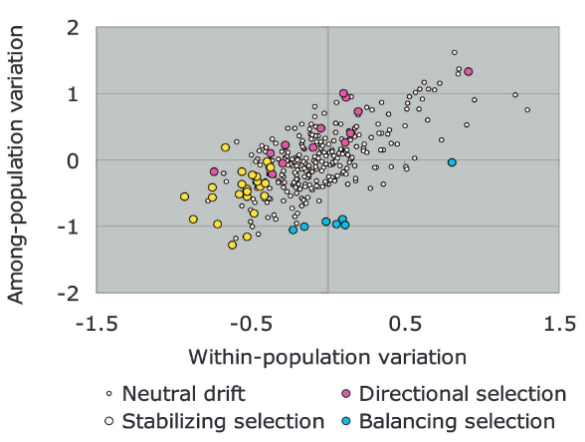
\includegraphics[width=0.8\textwidth, page=1] {figures/introduction/fig25.png}
    \caption[Variation de l'expression des gènes intra et inter-populations, indiquant différents modèles de divergence évolutive.]{
    \textbf{Variation de l'expression des gènes intra et inter-populations, indiquant différents modèles de divergence évolutive.}
     Les logarithmes de la variation de l'expression génique intra (abscisse) et inter population (ordonnée) sont représentés. En cas de dérive neutre, la variation intra-population est corrélée à la variation inter-population (cercles vide). D'autres gènes rejettent ce modèle nul. Les gènes soumis à une sélection directionnelle (cercles roses) ont été identifiés comme divergents le long d'un gradient de température de l'habitat après correction de la variance due à la phylogénie, et présentent une variation plus élevée entre les populations qu'au sein de celles-ci. Les gènes les plus influencés par la sélection stabilisante (cercles jaunes) ont une variation plus faible au sein des populations et entre elles que la plupart des gènes, et les gènes soumis à une sélection balancée (cercles bleus) ont une variation plus élevée au sein des populations qu'entre elles. Tirée de \citep{whitehead_neutral_2006}.\\
    }
    \label{fig:Fig25}
\end{figure} 

\subsubsection{Comparaison à plus grande échelle évolutive}
\label{subsec:comp-grande-echelle}

Le développement de techniques de mesure du transcriptome à haut débit a ensuite permis d’analyser l’évolution de l’expression des gènes à plus grande échelle évolutive. La difficulté n’est plus de capturer des transcrits suffisamment proches mais de pouvoir identifier correctement les isoformes d’un gène et les relations d’orthologies entre les gènes. Cela étant, la seconde difficulté est de normaliser correctement le niveau d’expression des gènes afin de pouvoir comparer les transcriptomes d’espèces distantes (cf \ref{subsec:expression-différentielle}). Ceci est habituellement fait en utilisant les gènes dont l’expression est la moins variable dans la grande majorité des tissus, comme les gènes dits de ménage. 

Brawand et collaborateurs ont analysé l’expression des gènes codants homologues de neuf espèces de mammifères et du poulet \citep{brawand_evolution_2011}. Ils ont montré que la divergence entre espèces des niveaux d’expression pour un même organe reflète correctement la distance génétique (Figure \ref{fig:Fig26}.A). Autrement dit, il est possible de retrouver la phylogénie de ces espèces en comparant les niveaux d’expression des gènes. Ceci confirme les travaux précédents montrant une accumulation des différences linéaires avec le temps de divergence (Figure 24). Cependant, cette divergence du niveau d’expression se stabilise à grande distance : la différence entre humain et poulet (ayant divergé il y a 300 millions d’années) est similaire à celle entre humain et opossum (160 millions d’années) (Figure \ref{fig:Fig26}.B). Cette observation suggère que la conservation des fonctions essentielles des organes pourrait définir une limite pour la divergence des transcriptomes. Cependant il pourrait aussi être simplement le fait d’une saturation du signal phylogénétique. 

\begin{figure}[h]
    \centering
    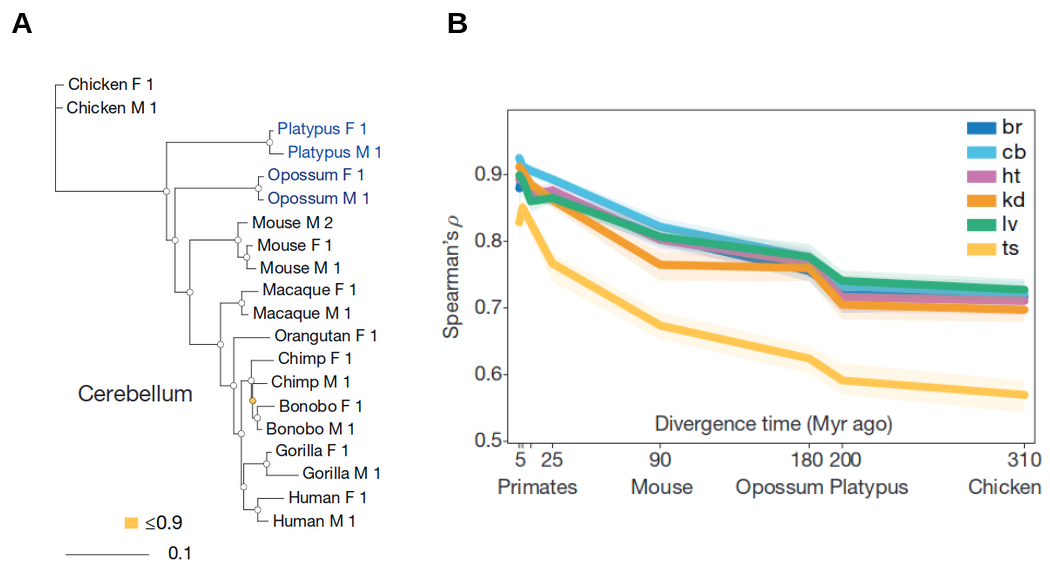
\includegraphics[width=1\textwidth, page=1] {figures/introduction/fig26.png}
    \caption[Corrélation des niveaux d'expression des gènes chez les vertébrés.]{
    \textbf{Corrélation des niveaux d'expression des gènes chez les vertébrés.}
    \textbf{A.} Phylogénie obtenue par Neighbour-Joining à partir de la corrélation de Spearman des niveaux d'expression dans le cervelet de l'ensemble de 5636 gènes orthologues 1-à-1 pour 10 espèces de vertébrés. Les valeurs de bootstrap (1000 tirages aléatoires avec remise) sont indiquées par des cercles blancs ($>$0.9) et jaune ($<$0.9).
    \textbf{B.} Corrélation de Spearman entre le niveau d'expression des gènes chez l'humain et 9 autres espèces selon le temps de divergence entre les espèces. Les enveloppes colorées autour des courbes indiquent les valeurs maximales et minimales de 100 réplicats de bootstraps. Tirée de \citep{brawand_evolution_2011}. \\
    }
    \label{fig:Fig26}
\end{figure} 

Cette étude montre également que les taux d’évolution des niveaux d'expression des gènes diffèrent entre les espèces étudiées. Ils sont plus élevés chez les primates que chez les rongeurs. L'évolution plus rapide de l'expression chez les primates s'explique probablement par une sélection moins efficace que par des changements adaptatifs plus fréquents. De par un temps de génération plus court, le nombre de mutations par unité de temps est plus élevé chez les rongeurs que chez les primates. On pourrait alors s’attendre à observer une plus grande divergence des niveaux d’expression chez les rongeurs que chez les primates, contrairement à ce qui a été observé. Néanmoins leur importante taille efficace de population permet l’élimination des mutations délétères \citep{ohta_slightly_1973}. Contrairement aux primates, qui ont des tailles de population réduites, et donc une sélection naturelle moins efficace. Cette observation est également en accord avec une analyse de l'évolution des séquences régulatrices, qui a révélé une évolution accélérée des éléments régulateurs chez les hominidés \citep{keightley_evidence_2005}. L’accumulation de mutations faiblement délétères entraîne une dérive des niveaux d’expression dans ces lignées.

\subsubsection{Evolution adaptative et biais potentiels}
\label{subsec:evol-adaptative}

L’étude de l’évolution de l’expression des gènes chez plusieurs espèces de vertébrés permet également de détecter des changements de niveaux d’expression qui pourraient être le résultat d’une évolution adaptative dans certaines lignées. Brawand et collaborateurs, ont ainsi modélisé l’évolution de l’expression des gènes le long de la phylogénie selon un modèle neutre et en prenant en compte la variabilité entre les individus de la même espèce \citep{brawand_evolution_2011}. Un niveau d’expression observé dans une lignée comme étant significativement différent de l’attendu selon ce modèle peut alors indiquer un changement d’optimum d’expression. Par exemple, le gène LIX1 ayant un rôle crucial dans le développement des neurones moteurs a été détecté comme significativement surexprimé dans le cerveau humain. Ou encore le gène COL25A1, lié à plusieurs pathologies neuronales et comportementales, est surexprimé chez les primates dans ce même organe (Figure \ref{fig:Fig27}). 

\begin{figure}[h]
    \centering
    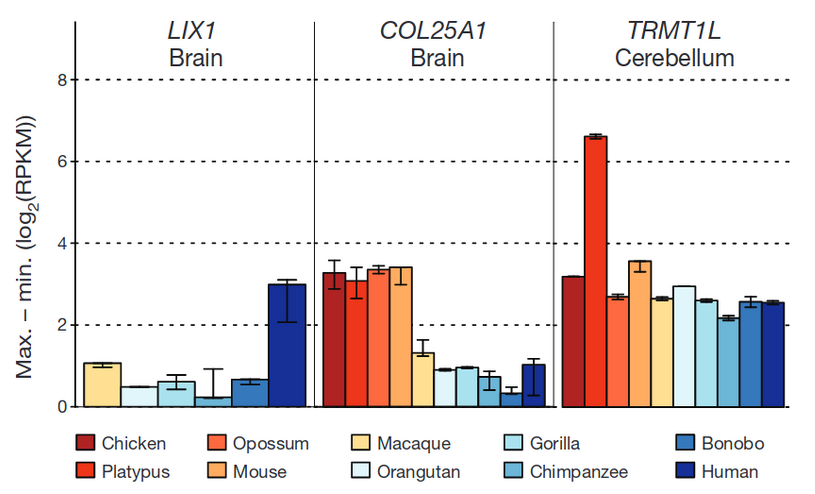
\includegraphics[width=0.8\textwidth, page=1] {figures/introduction/fig27.png}
    \caption[Changement de niveau d'expression spécifique d'une lignée.]{
    \textbf{Changement de niveau d'expression spécifique d'une lignée.}
    Exemple de gènes ayant évolué vers un nouvel optimum du niveau expression dans le cortex préfrontal chez l'humain (LIX1),  dans le cortex des primates (COL25A1) et dans le cervelet de l'ornithorynque (TRMT1L). Les barres d'erreurs représente l'étendue des valeurs d'expression au sein des différents individus d'une même espèce et tissu. Tirée de \citep{brawand_evolution_2011}.\\
    }
    \label{fig:Fig27}
\end{figure}

Il est cependant nécessaire de garder à l’esprit que de telles comparaisons sont empreintes de nombreux biais et facteurs confondants, et que les conclusions sur l’attribution de changement du niveau d’expression à la sélection adaptative doivent être prises avec précaution. Outre certains biais techniques précédemment évoqués (cf \ref{subsec:expression-différentielle}) pouvant affecter la mesure des niveaux d’expression, d’autres changements agissant à différentes échelles peuvent affecter les comparaisons. Par exemple, à l’échelle de la séquence, la recombinaison génétique peut entraîner un biais de fixation en faveur des nucléotides G et C, causant une accélération du taux d’évolution \citep{duret_biased_2009}. En agissant sur les éléments \gls{cis}-régulateurs, affectant alors le niveau d’expression des gènes cibles, ce biais peut alors être confondu avec un changement adaptatif \citep{capra_many_2013}. Aussi, en estimant le niveau d’expression d’un gène par la quantité de ses transcrits, on omet les nombreuses couches de régulation post-transcriptionnelle qui peuvent permettre de relâcher l’intensité de la sélection purifiante sur la quantité d’\acrshort{ARNm} \citep{wang_transcriptome_2020}. Un changement du niveau d’expression pourrait dans ce cas ne pas avoir d’effet sur le phénotype. En analysant le transcriptome sur des organes complets, il est également probable que des changements de la composition cellulaire spécifique d’une lignée puissent biaiser les comparaisons. L’estimation des niveaux d’expression des gènes à l’échelle cellulaire, notamment par du “single-cell \acrshort{RNA-seq}” pourraient permettre d’affiner ces comparaisons. Ces exemples de biais potentiels peuvent participer à la mauvaise interprétation de la part adaptative de l’évolution des niveaux d’expression.

\subsection{Variation de l’expression des gènes entre \glspl{condition}}
\label{sub:variation-condition}

Les variations du niveau d’expression des gènes entre espèces peuvent permettre de révéler des changements phénotypiques au sein d’un organe, cependant les gènes sont généralement exprimés dans plusieurs \glspl{condition}, au sein de différents tissus et stades de développement. Pour comprendre l’évolution de l’expression des gènes, il est nécessaire de comparer les transcriptomes au sein de ces différentes \glspl{condition}.

\subsubsection{Comparaison du niveau d’expression entre organes}
\label{subsub:variation-organes}

Les variations du niveau d’expression des gènes entre espèces peuvent permettre de révéler des changements phénotypiques au sein d’un organe, cependant les gènes sont généralement exprimés dans plusieurs \glspl{condition} et au sein de différents tissus. Pour comprendre l’évolution de l’expression des gènes, il est nécessaire de comparer les transcriptomes au sein de ces différentes \glspl{condition}. La comparaison des transcriptomes de dix espèces à travers six organes différents a révélé que les différences d’expression des gènes sont bien plus importantes entre les organes qu’entre les espèces (Figure \ref{fig:Fig28}) \citep{brawand_evolution_2011}. Par exemple l’expression des gènes est plus similaire entre le rein de l’humain et le rein du poulet qu’entre le rein et le cerveau d’une même espèce. Cette observation est attendue car la différenciation de ces tissus précède la divergence des espèces.

\begin{figure}[h]
    \centering
    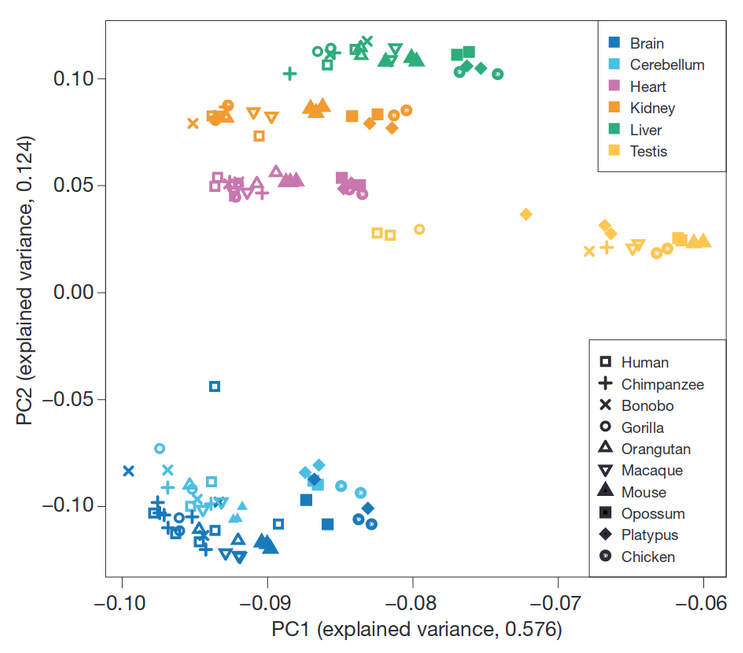
\includegraphics[width=0.8\textwidth, page=1] {figures/introduction/fig28.png}
    \caption[Comparaison des niveaux d'expression entre espèces et organes.]{
    \textbf{Comparaison des niveaux d'expression entre espèces et organes.}
    Analyse des Composantes Principales des niveaux d'expression de 5636 gènes orthologues 1-à-1 de plusieurs individus de 10 espèces de vertébrés au sein de 6 organes différents.
    Tirée de \citep{brawand_evolution_2011}.\\
    }
    \label{fig:Fig28}
\end{figure}

De plus, le taux d’évolution de l’expression des gènes est variable entre les tissus. Les testicules par exemple, dont l’évolution phénotypique est connue pour être rapide en raison de pression de sélection sexuelle liée à la compétition spermatique, présentent une évolution très rapide du niveau d’expression. Ceci peut donc s’expliquer par une sélection adaptative plus forte mais également par une plus faible sélection purificatrice liée à la présence de transcription non-fonctionnelle dans ces organes \citep{soumillon_cellular_2013}. A l’autre extrême, les tissus neuronaux présentent les taux de divergence d’expression les plus faibles. Bien que de nombreux changements phénotypiques aient eu lieu dans ces tissus, notamment la structure du cerveau, il semblerait que l’évolution de l’expression des gènes y soit très contrainte. Une plus forte sélection purificatrice sur leur activité pourrait être à l'œuvre. Aussi une plus grande spécialisation des types cellulaires composant les tissus neuronaux pourrait permettre d’affiner avec plus de précision l’activité des gènes et ne serait pas visible à l’échelle de l’organe entier. Un réseau de régulation d’expression plus robuste dans ces tissus pourrait également permettre de conserver une plus grande stabilité en limitant les effets délétères de mutations ponctuelles \citep{khaitovich_evolution_2006}.

\subsubsection{Comparaison du niveau d’expression entre stades de développement}
\label{subsub:variation-stade}

Afin de mieux comprendre l’évolution des traits phénotypiques entre les organismes, il peut également être important d’inclure une dimension temporelle de l’expression des gènes. Les changements de patron d’expression des gènes intervenant aux stades embryonnaires sont susceptibles d’être les plus pertinents d’un point de vue phénotypique. Dans une étude récente, Cardoso-Moreira et collaborateurs, ont séquencé les transcriptomes de sept espèces de vertébrés dans différents organes à plusieurs stades de développement comparables (Figure \ref{fig:Fig29}) \citep{cardoso-moreira_gene_2019}.

\begin{figure}[h]
    \centering
    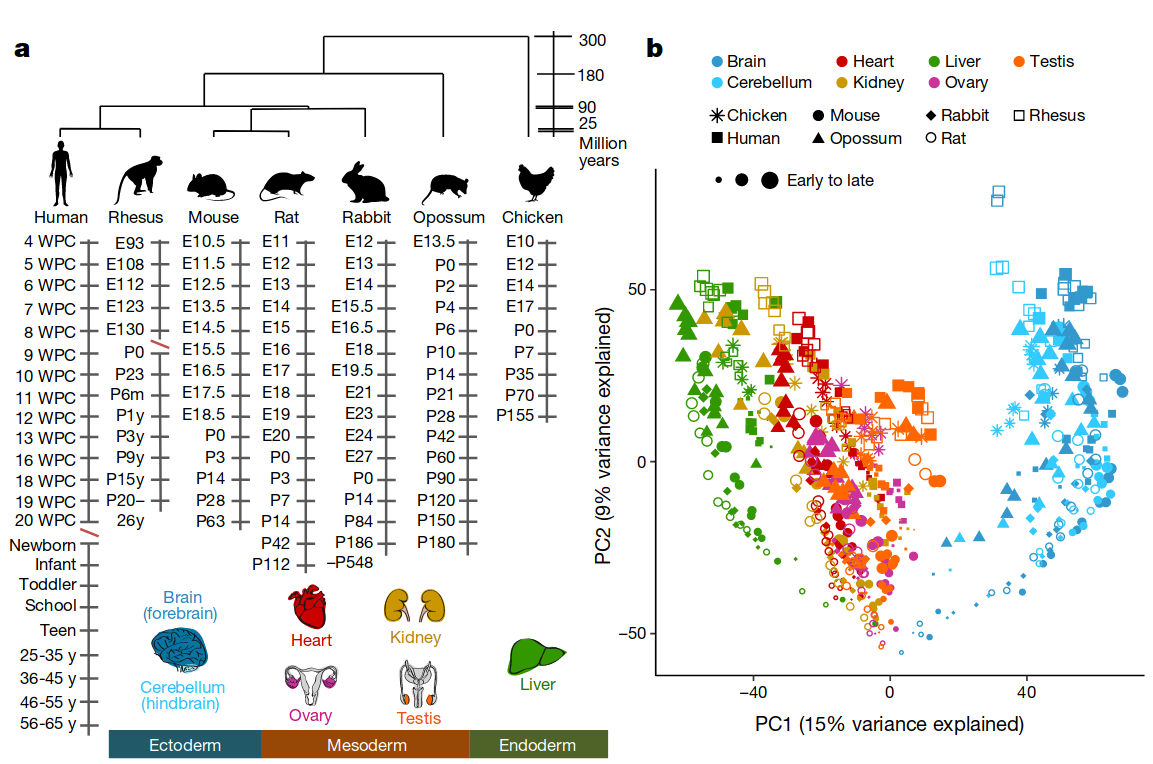
\includegraphics[width=1\textwidth, page=1] {figures/introduction/fig29.png}
    \caption[Transcriptomes de plusieurs organes à plusieurs stades de développement comparables de plusieurs espèces de vertébrés.]{
    \textbf{Transcriptomes de plusieurs organes à plusieurs stades de développement comparables de plusieurs espèces de vertébrés.}
    \textbf{A.} Espèces, organes et représentation des stades de développement alignés des échantillons analysés. \textbf{B.} Analyse des Composante Principale basée sur 7 696 gènes orthologues 1-à-1 dans toutes les espèces. Chaque point représente la médiane des réplicats techniques. Tirée de \citep{cardoso-moreira_gene_2019}.\\
    }
    \label{fig:Fig29}
\end{figure}

Comme précédemment, la différence entre les organes étudiés est la plus grande source de variabilité des patrons d’expression des gènes. Cependant, les échantillons prélevés dans des stades précoces quelle que soit l’espèce ou l’organe d’origine sont très similaires entre eux avant de diverger de manière progressive au cours du développement. Ceci peut s’expliquer par des modifications du nombre de \glspl{condition} dans lesquelles les gènes sont actifs. Au début du développement, les gènes actifs ont tendance à fonctionner dans de nombreux organes et stades, ce qui contraint leur évolution. Lorsque les organes se différencient et arrivent à maturité, les gènes actifs sont plus spécifiques avec des profils spatio-temporels plus restreints, ce qui peut réduire les contraintes fonctionnelles et faciliter les changements évolutifs. En effet, plus un gène est exprimé dans un grand nombre de tissus et plus son niveau d’expression est conservé \citep{khaitovich_evolution_2006}. Les contraintes évolutives agissant sur le niveau d’expression d’un gène augmentent avec le nombre de \glspl{condition} dans lesquelles le gène est exprimé. Si un gène est exprimé dans l’ensemble des tissus, le caractère délétère d’une mutation affectant son expression dans une seule \gls{condition} suffit pour la contre-sélectionner (Figure \ref{fig:Fig30}).

\begin{figure}[h]
    \centering
    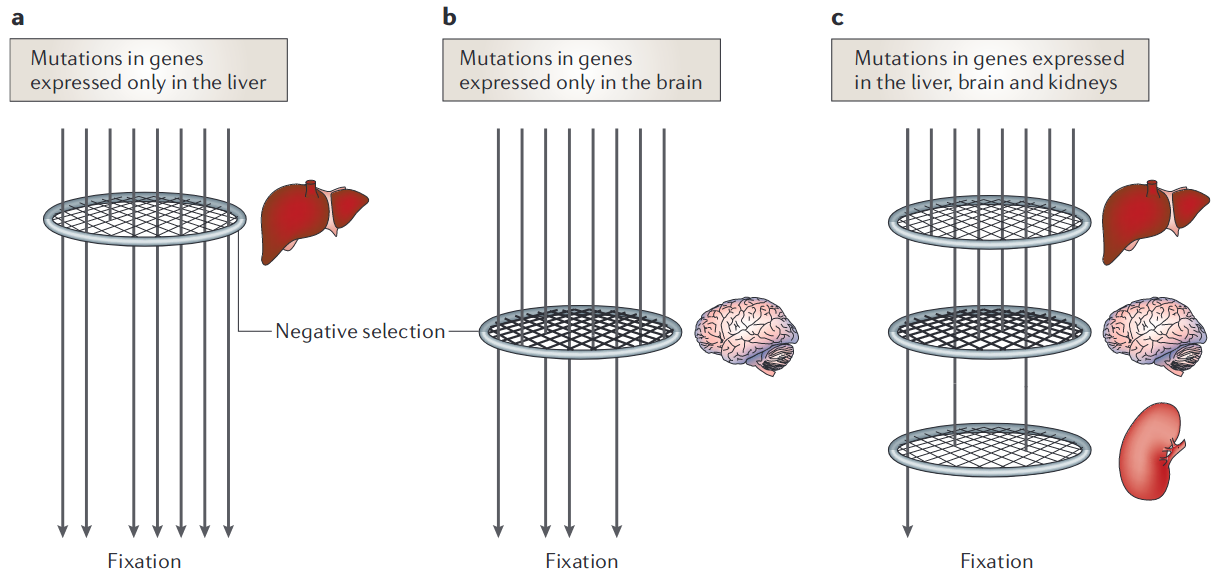
\includegraphics[width=0.9\textwidth, page=1] {figures/introduction/fig30.png}
    \caption[La sélection purifiante sur l'expression des gènes s'accumule avec le nombre de tissus.]{
    \textbf{La sélection purifiante sur l'expression des gènes s'accumule avec le nombre de tissus.}
    Plusieurs mutations affectent le niveau de l'expression des gènes exprimés uniquement dans le foie (\textbf{A}), uniquement dans le cerveau (\textbf{B}) et dans le foie, le cerveau et les reins (\textbf{C}). Les mutations  passent ou non le filtre de la sélection purifiante. Les niveaux d'expression des gènes dans le cerveau sont davantages contraints, une plus faible proportion de mutation arrive à fixation. Les contraintes s'additionnent avec le nombre de tissu dans lesquels un gène est exprimé, menant à une plus forte séléction purifiante. Tirée de \citep{khaitovich_evolution_2006}.\\
    }
    \label{fig:Fig30}
\end{figure}

\subsubsection{Evolution des profils d’expression}
\label{subsub:evol-profil}

Avec de telles données il est alors possible de mesurer des profils d’expression entre tissus et/ou au cours du développement, pour chaque gène indépendamment (Figure \ref{fig:Fig31}). Cela permet de comparer l’expression des gènes entre espèces distantes en s’affranchissant des procédures de normalisation visant à homogénéiser les niveaux d’expression des gènes. Les différences observées sont davantage qualitatives que quantitatives et permettent par exemple de déceler des changements majeurs de l’activité d’un gène dans un tissu ou encore des trajectoires temporelles d’expression. Par exemple, on a observé une réduction du niveau d’expression du gène GRIA3, important pour de nombreux processus neurophysiologiques, au cours du développement du cerveau humain, alors que pour les autres espèces l’expression de ce gène ne cesse d’augmenter (Figure \ref{fig:Fig31}) \citep{cardoso-moreira_gene_2019}. Inversement, le gène MDGA1, important pour le développement du système nerveux, est exprimé dans les stades précoces et diminue au cours du développement du cerveau chez de nombreuses espèces alors qu’elle s’active plus tardivement et augmente chez l’humain. Ces changements de trajectoire développementale sont de bons candidats pour expliquer certaines modifications phénotypiques au cours de l’évolution des mammifères.

\begin{figure}[h]
    \centering
    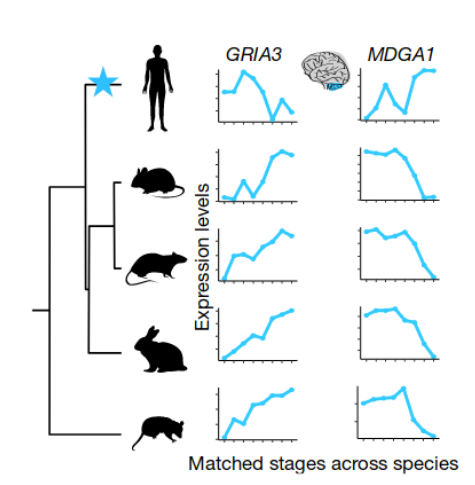
\includegraphics[width=0.6\textwidth, page=1] {figures/introduction/fig31.png}
    \caption[Evolution du profil temporel d'expression d'un gène.]{
    \textbf{Evolution du profil temporel d'expression d'un gène.}
    Exemple des profils temporels d'expression des gènes GRIA3 (récepteur de glutamate associé à la déficience intellectuel) et MDGA1 (glycoprotéine importante dans le développement du système nerveux) au cours du développement du cervelet à des stades de développement embryonnaire comparables chez quatre espèces. L'expression de ces gènes a évolué vers une trajectoires différente chez l'humain comparé aux autres espèces. Tirée de \citep{cardoso-moreira_gene_2019}.\\
    }
    \label{fig:Fig31}
\end{figure}

\subsection{Evolution de l’expression et de la séquence des gènes}
\label{sub:evol-exp-seq}

La vitesse d’évolution de l’expression des gènes est donc influencée par leur activité dans certains tissus ou stade de développement ainsi que par leur diversité fonctionnelle, c’est-à-dire leur rôle dans un grand nombre de contextes. Ces mêmes facteurs influencent également l’évolution des séquences \citep{kuma_functional_1995,hastings_strong_1996}. Il a ainsi été montré que le patron d’expression des gènes est un déterminant majeur des pressions de sélection agissant sur les régions codantes et non codantes des gènes \citep{duret_determinants_2000}. L’évolution de l’expression des gènes et des produits des gènes semblent en effet agir de manière parallèle. Les gènes exprimés dans un plus grand nombre de \glspl{condition} sont également ceux dont les séquences codantes présentent le moins de substitutions non-synonymes, indiquant une sélection purifiante plus importante à l’échelle de la séquence. De même que pour l’expression, les gènes actifs dans le cerveau sont ceux dont la séquence évolue le moins vite, à l’opposé de ceux exprimés dans les testicules (Figure \ref{fig:Fig32}) \citep{khaitovich_parallel_2005}. 

\begin{figure}[h]
    \centering
    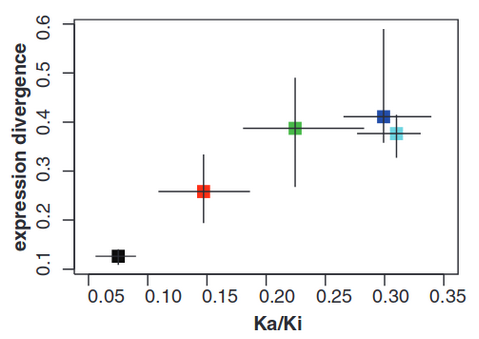
\includegraphics[width=0.7\textwidth, page=1] {figures/introduction/fig32.png}
    \caption[Corrélation entre la divergence d'expression et la divergence des séquences protéiques entre l'humain et le chimpanzé.]{
    \textbf{Corrélation entre la divergence d'expression et la divergence des séquences protéiques entre l'humain et le chimpanzé.} La divergence d'expression est mesurée par la différence médiane entre les niveaux d'expression normalisés des gènes exprimés dans les deux espèces dans le cerveau (noir), le coeur (rouge), les reins (vert), le foie (bleu foncé) et les testicules (bleu clair). La divergence de séquence protéique est mesuré par le nombre de substitutions non-synonyme par site non-synonyme (Ka) normalisé par le nombre de substitution par site dans une fenêtre de 250kb autour du centre du gène (Ki). Les tissus qui présentent une forte divergence de séquence d'acides aminés ont tendance à présenter une forte divergence d'expression (r de Pearson = 0,94, P $<$ 0,05). Les barres d'erreur représentent les intervalles de confiance à 95\% des valeurs médianes calculées à partir de 10 000 réplicats de bootstrap. De \citep{khaitovich_parallel_2005}.\\
    }
    \label{fig:Fig32}
\end{figure}

De plus, la corrélation positive entre la divergence des séquences codantes et de l’expression des gènes semble constante quelque soit la distance évolutive \citep{warnefors_evolution_2013}. Certaines catégories de gènes semblent néanmoins échapper à cette règle générale. Par exemple, les gènes impliqués dans le développement ou ayant des fonctions neuronales ont tendance à avoir une évolution de l’expression accélérée par rapport à l’évolution de leurs séquences. Les gènes impliqués dans des fonctions immunitaires ou associés à la reproduction mâle ont quant à eux une évolution de leur expression plus rapide de leur séquence protéique \citep{haygood_contrasts_2010}.

\section{Evolution de la régulation de l’expression des gènes}
\label{sec:evol-regul}

L’évolution de l’expression des gènes entre espèces et entres \glspl{condition} implique des variations des mécanismes de régulation sous-jacents. Comme nous l’avons vu ces derniers peuvent être nombreux et complexes (cf \ref{chap:regulation-de-expression}). L’étude de l’évolution de la régulation de l’expression des gènes peut ainsi s’établir à plusieurs niveaux. Je détaillerai ici les bases moléculaires de l’évolution de l’expression agissant au niveau des séquences \gls{cis}-régulatrices via des modifications épigénétiques et génétiques.

\subsection{Variations épigénétiques}
\label{subsec:variation-epigenet}

Les variations épigénétiques, comme la modification des histones ou la méthylation de l’ADN affectent la structure de la chromatine et peuvent alors impacter les repliements et/ou l’accessibilité de l’ADN. De telles modifications sont susceptibles d’avoir des conséquences sur la fixation des \acrshort{FT}s ou de la polymérase II sur les éléments régulateurs, modifiant l’expression des gènes concernés. La relation de cause à effet n’est pas évidente car inversement l’activation de la transcription induit également la pose de certaines marques épigénétiques comme H3K27ac sur le promoteur, l’\gls{amplificateur} et le corps du gène pour stabiliser l’ouverture de la chromatine. Les changements épigénétiques peuvent être héritables et pourraient alors expliquer une part importante des variations de l’expression des gènes entre espèces sans affecter la séquence d’ADN en elle-même \citep{lind_evolutionary_2018}. \\

Par exemple, Cain et collaborateurs ont comparé les marques de méthylation d’histone H3K4me3, associées à une augmentation de la transcription, sur des cellules lymphoblastoïdes de plusieurs primates \citep{cain_gene_2011}. Ils ont observé une forte conservation de la position de ces marques mais un enrichissement significatif des différences de H3K4me3 sur les \acrshort{TSS} des gènes différentiellement exprimés. La présence supplémentaire d’une marque H3K4me3 proche d’un gène est associée à une augmentation de son niveau d’expression et inversement lorsque la marque n’est pas observée. Bien que la relation de cause à effet n'ait pas été prouvée, les variations de H3K4me3 pourraient expliquer jusqu’à 7\% des différences d’expression des gènes entre l’humain et le chimpanzé dans ces cellules. Une autre étude a confirmé ces résultats et les a complété avec plusieurs autres marques épigénétiques (H3K4me1, H3K4me3, H3K27ac et H3K27me3) et la présence de l’ARN polymérase II chez plusieurs primates \citep{zhou_epigenetic_2014}. Chacune des marques étudiées est associée à des différences de niveau d’expression des gènes voisins. Prises ensemble elles expliqueraient près de 40\% de la variance des niveaux d’expression des gènes dans les cellules lymphoblastoïdes. En combinant l’analyse de ces marques avec une mesure d’accessibilité de la chromatine (ATAC-seq, cf \ref{subsubsec:ouverture-chroma}), il a également été montré que les variations épigénétiques entre les primates semblent associée à l’activité des éléments \gls{cis}-régulateurs \citep{garcia-perez_epigenomic_2021}. Les promoteurs des gènes sont les moins sujets à ces variations alors que les \glspl{amplificateur} actifs présentent des marques épigénétiques les plus divergentes. \\

La méthylation de l’ADN au niveau des cytosines des dinucléotides \acrshort{CpG} est également un facteur important pour l’expression des gènes. Enrichies au niveau de certains promoteurs des gènes, ces dinucléotides peuvent être hyper-méthylés et ainsi modifier les interactions avec d’autres protéines ce qui réduit le niveau d’expression des gènes associés \citep{jones_role_2001}. Cette marque épigénétique peut également être héritable et contribuer à la divergence des niveaux d’expression entre espèces. Entre 11\% à 25\% des gènes différentiellement exprimés entre l’humain et le chimpanzé pourrait être la conséquence de variations de méthylation de l’ADN sur leur promoteur \citep{pai_genome-wide_2011, blake_comparison_2020}. De plus, la divergence de méthylation sur les promoteurs est également associée positivement à la divergence des séquences codantes, ce qui comme précédemment évoqué indiquerait une évolution parallèle entre la régulation et les produits des gènes \citep{hernando-herraez_dynamics_2013}. \\

Cependant ces associations entre modifications épigénétiques et divergence de l’expression ne sont pas nécessairement le reflet de causalité directe et n’excluent pas la part importante des variations au niveau génétique. Des changements sur les sites de fixation des \acrshort{FT}s pourraient notamment être le déterminant majeur des différences de l’état de la chromatine entre les espèces \citep{mcvicker_identification_2013}.

\subsection{Evolution du répertoire des éléments \gls{cis}-régulateurs}
\label{subsec:evol-repertoire}

Les éléments \gls{cis}-régulateurs dans les génomes peuvent varier en nombre, par des gains ou des pertes de séquence et alors entrainer des variations importante de l’expression des gènes. L’émergence de nouveaux éléments \gls{cis}-régulateurs peut survenir par l’apparition de nouveaux sites de fixation de facteur de transcription, qui à leur tour pourront avoir un impact sur la transcription du gène. Ces éléments pourraient premièrement émerger de novo à partir de mutations ponctuelles sur des séquences non-régulatrices. De telles régions régulatrices de novo ont été identifiées dans les génomes de poissons téléostéens à partir d’anciennes copies dupliquées et dégénérées de gènes codants \citep{eichenlaub_novo_2011}. Cependant, il peut être difficile d’identifier des régions orthologues sur des séquences non-codantes pouvant évoluer rapidement. Il est ainsi délicat de déterminer si ces éléments \gls{cis}-régulateurs sont réellement apparus de novo ou à partir d'élément régulateur ancestral ayant divergé suffisamment pour ne plus être identifiable dans d’autres lignées. Deuxièmement, les duplications ou transpositions à partir d’éléments \gls{cis}-régulateurs ancestraux semblent être des mécanismes majeurs dans l’apparition de nouvelles fonctions régulatrices \citep{rebeiz_enhancer_2018}. Chez plusieurs espèces de drosophiles par exemple, 7 \glspl{amplificateur} du gène shavenbaby semblent provenir de la duplication à répétition d'une séquence régulatrice ancestrale  (Figure \ref{fig:Fig33}) \citep{kittelmann_complex_2021}. Ces différentes copies d’\glspl{amplificateur} ont évolué vers une sous-fonctionnalisation pour activer l’expression de shavenbaby de manière spécifique dans différentes cellules de l’embryon de Drosophila melanogaster. Ces duplications réduisent la pléiotropie de l’élément \gls{cis}-régulateur unique ancestral et faciliteraient l’évolution de nouveaux patrons d’expression du gène \citep{murugesan_evolution_2022}. \\

\begin{figure}[h]
    \centering
    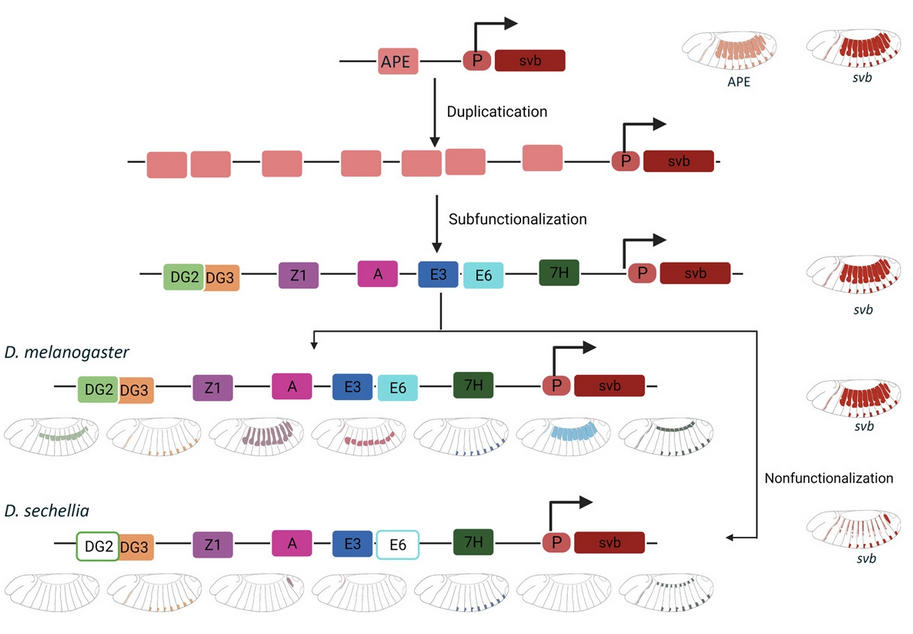
\includegraphics[width=0.8\textwidth, page=1] {figures/introduction/fig33.png}
    \caption[Scénario probable de l'évolution des éléments \gls{cis}-régulateurs du gène \textit{shavenbaby} chez les drosophiles.]{
    \textbf{Scénario probable de l'évolution des éléments \gls{cis}-régulateurs du gène \textit{shavenbaby} chez les drosophiles.}
    Un unique amplificateur ancestral pléiotropique (APE) régule l'expression du gène \textit{shavenbaby} (\textit{svb}) dans plusieurs régions de l'embryon chez l'ancêtre commun de plusieurs lignées de drosophiles. APE est dupliqué en sept copies dans les génomes des descendants et évolue vers une sous-fonctionnalisation. Chez \textit{Drosophila melanogaster} chaque copie active l'expression de \textit{svb} dans des régions différentes de l'embryon. Chez \textit{D. sechellia}, certaines copies perdent leur fonction et provoque l'inactivation de \textit{svb} dans certaines régions de l'embryon. Tirée de \citep{murugesan_evolution_2022} à partir de l'étude de \citep{kittelmann_complex_2021}.\\
    }
    \label{fig:Fig33}
\end{figure}

La perte totale ou partielle de la séquence des éléments \gls{cis}-régulateur peut de la même manière participer à des changement d’expression des gènes et à l’évolution phénotypique. Chez Drosophila sechellia, la perte de la fonction régulatrice de 2 des 7 éléments \gls{cis}-régulateurs de shavenbaby élimine ainsi son expression dans certaines cellules et entraine un changement de la morphologie de la cuticule chez cette espèce (Figure \ref{fig:Fig33}) \citep{kittelmann_complex_2021}. D’autres exemples existent chez les vertébrés, comme la délétion d’un \gls{amplificateur} du gène codant pour le récepteur à l’androgène qui pourrait être à l’origine de la perte des vibrisses (moustache sensorielle) et des épines péniennes chez l’humain \citep{mclean_human-specific_2011}. Chez les cétacés, la réduction des membres inférieurs pourrait être en partie expliquée par plusieurs délétions et substitutions sur un \gls{amplificateur} du gène Tbx4 qui engendreraient une diminution de son expression et ainsi une réduction du développement des membres \citep{liang_divergence_2022}. \\

Il toutefois important de noter que les délétions peuvent également être à l’origine de gain phénotypique en supprimant des éléments \gls{cis}-régulateurs répresseurs de l’expression des gènes. Inversement, une perte phénotypique peut être la conséquence d’un gain d’activité de gènes qui contrôlent les patrons de développement, tels que la prolifération, la mort ou la migration des cellules. C’est par exemple le cas du gain d’activité du gène Bmp4, contrôlant notamment l’apoptose, qui pourrait être lié à la perte du phallus chez le poulet. Exemple que j’aborderai plus en détail dans le Chapitre 4 (cf partie \ref{chap:4-evolpheno}) \citep{herrera_developmental_2013}.

\subsection{Evolution des séquences des éléments \gls{cis}-régulateurs}
\label{subsec:evol-seq-regul}

Plusieurs études ont montré l’importance des mutations des régions régulatrices sur les variations phénotypiques au niveau morphologique, physiologique et comportemental \citep{wray_evolutionary_2007}. Des mutations survenant sur ces séquences peuvent modifier les motifs reconnus par les éléments régulateurs agissant en trans comme les \acrshort{FT}s. Schmidt et collaborateurs ont analysé l’occupation de deux \acrshort{FT}s dans le foie de cinq espèces de vertébrés \citep{schmidt_five-vertebrate_2010}. Malgré une reconnaissance de motifs très conservés, les sites de fixation de ces \acrshort{FT} sont très variables entre espèces. Cette différence de fixation est expliquée par la divergence de séquence des éléments \gls{cis}-régulateurs actifs dans ce tissu. A l’inverse, le facteur de transcription CTCF, qui a un rôle important dans l’organisation tridimensionnelle du génome, possède des sites de fixation très fortement conservés entre espèces de vertébrés \citep{schmidt_waves_2012}. Ceci indique une variabilité importante des pressions de sélection agissant sur les sites de fixation. Entre l’humain et le chimpanzé, qui partagent une forte similarité de séquence, les sites de fixation de l’ARN polymérase II sont largement partagés. Cependant près de 32\% d’entre eux montrent une différence quantitative de la présence de l’ARN polymérase sur leurs séquences \citep{kasowski_variation_2010}. Cette différence est expliquée par des mutations d’un seul nucléotide (SNP) ou des variations structurelles comme des inversions qui pourraient modifier l’affinité de l’ARN polymérase II avec ces sites. De plus, les changements de fixation de cette polymérase sont corrélés avec les divergences des niveaux d’expression de plusieurs gènes entre l’humain et le chimpanzé.

\subsubsection{Evolution des séquences promotrices}
\label{subsubsec:evol-seq-promo}

Au niveau des séquences des promoteurs, le taux d’évolution semble être très variable entre gènes mais aussi entre les espèces \citep{taylor_heterotachy_2006}. En analysant les taux d’évolution neutre de manière locale pour éviter les biais de fixation, des études montrent que la divergence de certains promoteurs pourrait être le fruit d’une évolution adaptative chez l’humain \citep{haygood_promoter_2007, torgerson_evolutionary_2009}. Notamment, l’évolution de ces séquences promotrices pourrait être responsable de changement d’expression de gènes impliqués dans des processus du développement du cerveau et du système nerveux. Dans des espèces où la sélection purifiante est plus efficace comme chez les souris, l’évolution des séquences \gls{cis}-régulatrices pourrait également être associés à une plus grande part de sélection positive et adaptative que les séquences codantes \citep{halligan_contributions_2013}.

\subsubsection{Evolution des séquences des \glspl{amplificateur}}
\label{subsubsec:evol-seq-enh}

Une comparaison des profils de fixation des facteurs de transcription entre la souris et l’humain a montré que les sites de fixation présents sur les promoteurs sont davantage conservés que ceux présents sur les \glspl{amplificateur} distaux \citep{cheng_principles_2014}. La majorité des éléments \gls{cis}-régulateurs, particulièrement les \glspl{amplificateur} semblent subir une évolution très rapide de leur séquence chez l’ensemble des mammifères (réf?). Il existe cependant des variations dans le taux d’évolution. Certains sont très conservés et régulent des processus fondamentaux tissu-spécifiques \citep{ballester_multi-species_2014} ou sont actifs dans de nombreux tissus \citep{cheng_principles_2014}. D’autres sont beaucoup plus variables et pourraient être associés à des gènes sous sélection positive (réf?). 

Par exemple, la séquence et l’activité de l’\gls{amplificateur} \acrshort{ZRS} sont très fortement conservés à l’échelle des vertébrés \citep{kvon_progressive_2016}. Ceci s’explique par une forte pression purifiante car comme nous l’avons vu précédemment les effets de certaines mutations sur \acrshort{ZRS} sont très fortement délétères sur l’expression de \acrshort{SHH} et le développement des membres. Cependant chez les serpents, des tétrapodes qui ont perdu leurs membres, cet \gls{amplificateur} a subi une accumulation de mutations dont d’importantes délétions. Le remplacement par transgénèse du \acrshort{ZRS} de la souris par la séquence homologue du python entraîne une réduction importante des membres, signe de la perte de sa fonction régulatrice sur \acrshort{SHH} (Figure \ref{fig:Fig34}). La régénération artificielle d’un seul site de fixation très conservé chez les vertébrés sur la séquence de \acrshort{ZRS} du python résulte en un regain d’activité de \acrshort{SHH} et permet le développement normal des membres chez la souris (Figure \ref{fig:Fig34}.B) \citep{lettice_opposing_2012}. Cette variation de quelques nucléotides souligne l’importance de l’évolution des \glspl{amplificateur} pour la divergence phénotypique. 

\begin{figure}[h]
    \centering
    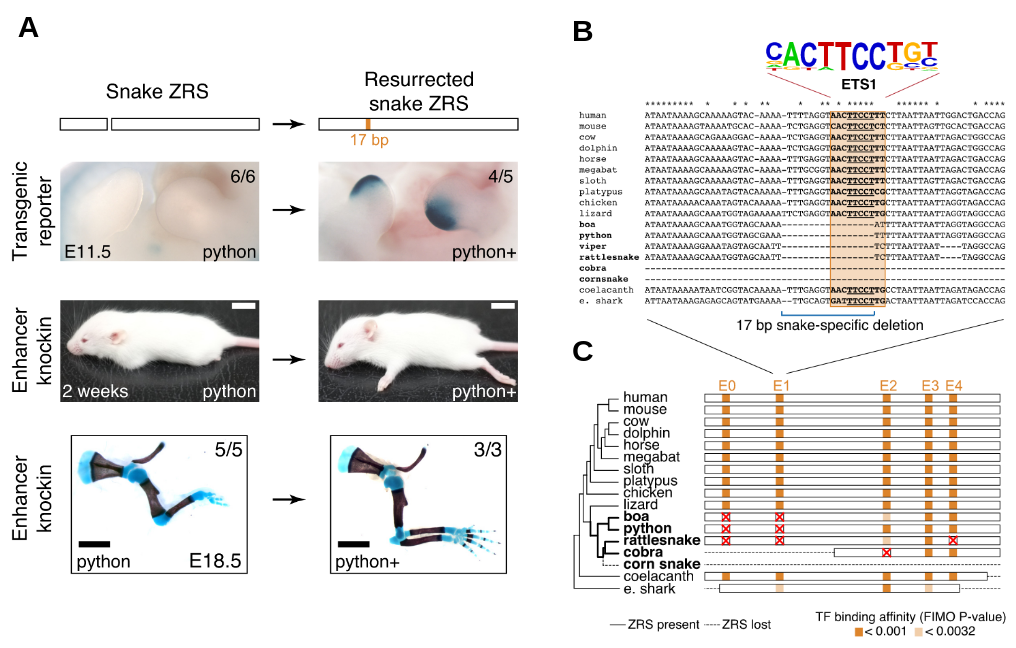
\includegraphics[width=1\textwidth, page=1] {figures/introduction/fig34.png}
    \caption[Résurrection \textit{in vivo} de la fonction de l'amplificateur \acrshort{ZRS} du python.]{
    \textbf{Résurrection \textit{in vivo} de la fonction de l'amplificateur \acrshort{ZRS} du python.}
    \textbf{A.} A gauche : transgénèse de l'\gls{amplificateur} \acrshort{ZRS} du python dans une souris. A droite : transgénèse de l'\gls{amplificateur} \acrshort{ZRS} du python édité pour inclure 17 paires de base très conservées chez les vertébrés dans une souris. De haut en bas : Activité \textit{in vivo} du \acrshort{ZRS} intégré dans les bourgeons des membres d'une souris au stade embryonnaire E11.5. Le gène rapporteur LacZ permet de colorer les cellules lorsque \acrshort{ZRS} est actif. Phénotype de la souris au bout de 2 semaines. Radio du membre de la souris au stade embryonnaire E18.5. 
    \textbf{B.} Alignement d'une partie de la séquence de \acrshort{ZRS} de plusieurs vertébrés. Les 17 paires de bases perdues chez les serpents contiennent un motif reconnu par le facteur de transcription ETS1. 
    \textbf{C.} Distribution des sites de fixation de ETS1 sur la séquence de \acrshort{ZRS} chez les vertébrés. Les croix rouges indiquent la perte du motif. Tirée de \citep{kvon_progressive_2016}. \\
    }
    \label{fig:Fig34}
\end{figure}

De plus, la modification de la séquence des éléments \gls{cis}-régulateurs peuvent participer à l’émergence de nouvelle fonction. Chez plusieurs espèces de drosophiles, l’expression convergente du gène yellow, notamment responsable du patron de coloration, est par exemple fortement dépendante de quelques éléments \gls{cis}-régulateurs \citep{prudhomme_repeated_2006}. Chez deux espèces, plusieurs substitutions sur deux éléments \gls{cis}-régulateurs entraînent un gain d’expression du gène dans plusieurs tissus et une coloration convergente. Inversement, la perte convergente de cette coloration chez deux autres espèces serait liée à des mutations faisant perdre l'activité d’un même \gls{amplificateur} de yellow. Un autre exemple est celui de HACNS1 qui est un élément \gls{cis}-régulateur fortement conservé chez les vertébrés terrestres et actif dans le développement de nombreuses structure. Plusieurs substitutions sur sa séquence permettent un gain de fonction qui semble spécifique à la lignée humaine \citep{prabhakar_human-specific_2008}. Cette nouvelle activité pourrait notamment être liée à l’adaptation morphologique caractéristique des doigts des mains chez l’humain, comme la présence d’un pouce opposable. Le gain de fonction régulatrice à partir de l’évolution d’éléments \gls{cis}-régulateurs ancestraux est ainsi probablement un mécanisme important dans l’adaptation morphologique des espèces \citep{koshikawa_enhancer_2015}.

\subsection{Activité des éléments \gls{cis}-régulateurs}
\label{subsec:evol-seq-enh}

L’activité des éléments \gls{cis}-régulateurs, c’est-à-dire leur capacité à réguler l’expression de gènes, au sein des différentes \glspl{condition} cellulaires est egalement un facteur important à prendre en considération. Leur patron d’activité peut en effet être modifié et alors impacter l’expression des gènes cibles indépendamment de la divergence de leur séquence. Des modifications épigénétiques, comme l’accessibilité de la chromatine ou les modifications d’histones, peuvent ainsi être à l’origine de gain d’activité d’élément \gls{cis}-régulateur existant ce qui impacte l’expression des gènes cibles dans de nouveau tissu ou contexte cellulaire \citep{rebeiz_evolutionary_2011, xin_enhancer_2020}. \\

L’activité de la majorité des éléments \gls{cis}-régulateurs évolue très rapidement chez les mammifères \citep{xiao_comparative_2012, cotney_evolution_2013, villar_enhancer_2015}. L’activité mesurée par la présence de marques épigénétiques H3K27ac (\gls{amplificateur} actif) et H3K4me3 (promoteur actif) dans le foie de vingt espèces montre ainsi que plus de la moitié des \glspl{amplificateur} dont les séquences sont alignables sont actifs dans une seule espèce \citep{villar_enhancer_2015}. Ceci représente environ 10 000 éléments uniques à chacune des espèces étudiées. L’activité des promoteurs quant à eux est majoritairement conservée chez ces espèces, en accord avec l’évolution plus lente de leur séquence évoquée précédemment \citep{cheng_principles_2014}. Les \glspl{amplificateur} espèce-spécifiques semblent avoir évolué au sein de chaque lignée majoritairement à partir de séquences d’ADN ancestrales non-codantes déjà présentes \citep{villar_enhancer_2015}. Le gain d’activité par des modifications épigénétiques pourrait également permettre de moduler différemment les niveaux d’expression. En effet de tels gains d’activité des \glspl{amplificateur} sont associés avec l’augmentation des niveaux d’expression dans le développement des membres de l’humain par rapport au macaque \citep{cotney_evolution_2013}. \\

Comme nous l’avons vu pour \acrshort{SHH} et \acrshort{ZRS}, un élément \gls{cis}-régulateur crucial d’un gène peut se localiser dans l’intron d’un autre gène. Cette structure peut fortement contraindre la localisation des deux gènes pour se maintenir en synténie, c'est-à-dire en proximité sur la séquence. Dans une étude récente, Wong et collaborateurs ont analysé des paires de gènes voisins dont la synténie est fortement conservée à l’échelle des métazoaires \citep{wong_deep_2020}. Ils ont ainsi pu associer certains \glspl{amplificateur} présents dans ces régions en micro-synténie dans le génome de l’éponge (Amphimedon queenslandica) à des \glspl{amplificateur} situés dans des régions orthologues chez des vertébrés. Les séquences de ces \glspl{amplificateur} sont fortement divergentes mais ceux-ci présentent une forte conservation d’activité mesurée par la marque H3K4me1. La transgénèse d’un de ces \glspl{amplificateur} de l’éponge avec un gène indicateur de son activité (Green Fluorescent Protein ou \acrshort{GFP}) dans le génome du poisson-zèbre a montré un patron d’activité cellule-spécifique similaire à celui de l’\gls{amplificateur} du poisson-zèbre de la région micro-synténique orthologue. Ceci indique que les \acrshort{FT}s du poisson-zèbre reconnaissent des sites de fixation sur cet \gls{amplificateur}. En analysant le nombre et la diversité des \acrshort{FT}s se fixant sur les \glspl{amplificateur} de l’éponge dans des régions micro-synténique, cette étude a permis de proposer des \glspl{amplificateur} orthologues chez le poisson-zèbre, la souris et l’humain conduisant à des patrons d’activité similaires. Ainsi certains éléments \gls{cis}-régulateurs pourraient subir une forte divergence de séquence mais conserver leur fonctionnalité en fixant une configuration similaire de \acrshort{FT}.

\subsection{Réarrangements génomiques}
\label{subsec:rearrangement}

La présence d’interactions régulatrices à longue distance entre les promoteurs des gènes et les éléments \gls{cis}-régulateurs suggère que les réarrangements génomiques peuvent avoir un rôle important dans l’évolution de l’expression des gènes. Ces mutations à grande échelle, telles que les délétions, duplications, inversions et translocations de segments chromosomiques, impliquent une réorganisation importante des génomes. Grâce à des approches comparatives ou par des expériences de transgénèse, il est possible d’étudier l’effet des réarrangements sur l’évolution de l’expression des gènes. C’est notamment par le biais de délétions et d’inversions induites sur des embryons de souris que les premières études ont permis de décrire la structure des paysages régulateurs des gènes du développement \citep{tschopp_genetic_2011}. \\

Des réarrangements qui perturbent le contact entre le promoteur de \acrshort{SHH} et son \gls{amplificateur} \acrshort{ZRS}, provoquent des changements importants de l’expression du gène et ont des conséquences phénotypiques sur le développement des membres (Figure \ref{fig:Fig35}) \citep{symmons_SHH_2016}. En faisant varier la distance entre ces deux régions grâce à des séries de délétions et inversions dans des génomes de souris, cette étude a cherché à caractériser les limites de l’action de \acrshort{ZRS} sur \acrshort{SHH}. Dans la mesure où les deux loci restent à l’intérieur d’un certain domaine (ou \acrshort{TAD}, cf \ref{subsubsec:TAD-boucle}), la distance qui les sépare n’a pas d’influence significative sur l’expression du gène. Cependant en dehors de ce domaine, plus la distance qui sépare \acrshort{ZRS} du promoteur de \acrshort{SHH} est grande et moins le gène est exprimé. Ceci peut s’expliquer par une diminution de la probabilité de contact entre les deux régions. La rupture de la relation régulatrice résulte alors en un développement anormal des membres. Cette étude permet également de démontrer que l’organisation spatiale de l’ADN peut permettre de relâcher une partie de la contrainte de proximité génétique entre deux régions devant être physiquement proches pour fonctionner. Tant que le repliement de la chromatine permet une proximité ou “synténie spatiale”, une certaine variabilité de distance serait permise entre un gène et ses éléments \gls{cis}-régulateurs. Des régions distantes dans le génome humain mais proches dans celui de la souris, ont ainsi une plus grande probabilité d’être en contact dans les cellules humaines qu’attendu par hasard \citep{veron_close_2011}.

\begin{figure}[h]
    \centering
    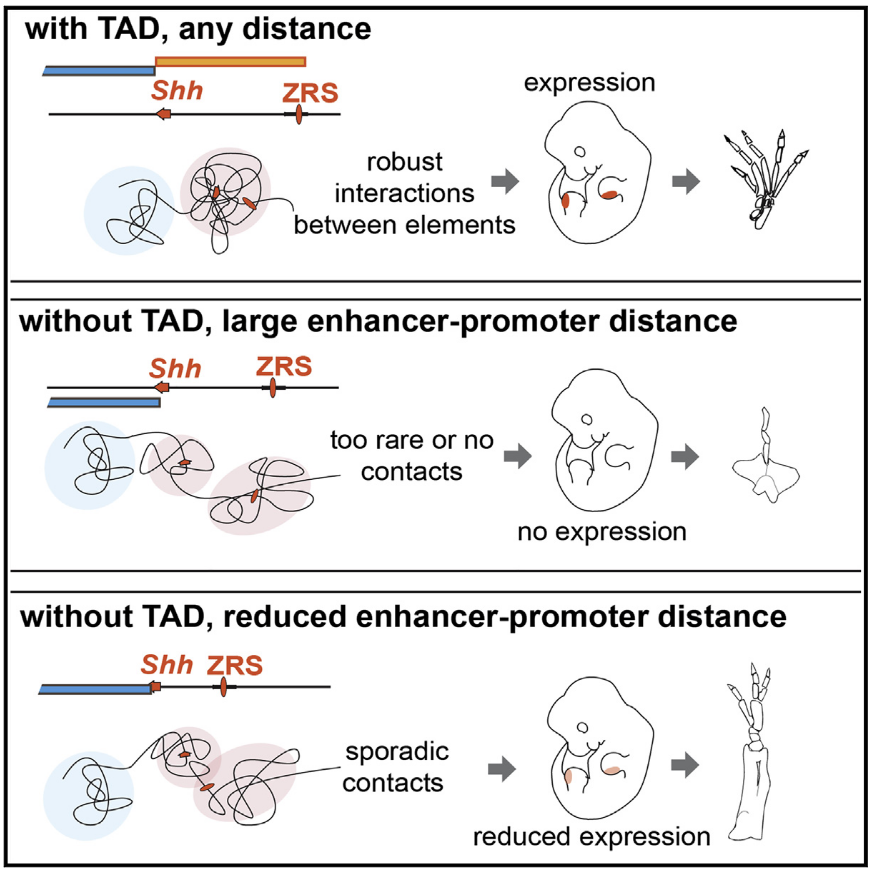
\includegraphics[width=0.7\textwidth, page=1] {figures/introduction/fig35.png}
    \caption[Schéma bilan des conséquences de réarrangements génomiques entre Shh et ZRS.]{
    \textbf{Schéma bilan des conséquences de réarrangements génomiques entre Shh et ZRS.}
    Des délétions et inversions sont induites entre les deux loci dans les génomes d'embryons de souris. \textbf{En haut}, Shh et ZRS restent localisés dans le même domaine d'association topologique (TAD). Quelque soit la distance génomique qui les sépare, les deux régions sont en proximité physique dans le noyau, l'expression de Shh dans le bourgeon des membres est inchangée et la formation des membres est normale. \textbf{Au milieu}, Shh et ZRS sont séparés par une grande distance génomique et ne sont plus localisés dans le même TAD. Les contacts de chromatine entre les régions sont rares, Shh n'est pas exprimé dans le bourgeon des membres et les membres sont tronqués. \textbf{En bas}, Shh et ZRS sont séparés par une faible distance génomique mais ne sont pas dans le même TAD. Des contacts sporadiques de la chromatine sont observés entre les loci, Shh est exprimé à un faible niveau, les membres se développent avec des malformations. 
    Tiré de \citep{symmons_SHH_2016}. \\
    }
    \label{fig:Fig35}
\end{figure}

Un réarrangement peut également engendrer l’adoption d’un élément \gls{cis}-régulateur par un gène, comme il semblerait être le cas pour une malformation des membres chez l’humain \citep{lettice_enhancer-adoption_2011}. Chez un individu atteint de cette maladie, suite à une inversion d’une région de plus de 500kb, le gène \acrshort{SHH} est relocalisé. En imitant cette inversion dans le génome de la souris, le gène \acrshort{SHH} est exprimé de façon anormale dans le cerveau et dans les membres et ne semble plus sous le contrôle de \acrshort{ZRS}. Cependant, \acrshort{SHH} est tout de même actif dans le bourgeonnement des membres. Il présente un patron d’expression similaire aux gènes normalement contrôlés par un autre élément \gls{cis}-régulateur fortement conservé et actif dans les membres nommé HCNE2. Bien que la présence d’un contact n'ait pas été testé, le rapprochement de \acrshort{ZRS} à 190kb de HCNE2 suite à cette inversion semble contrôler l’expression anormale du gène dans ce tissu. \\

En comparant conjointement l’organisation des génomes et l’expression des gènes dans le cerveau de l’humain et du chimpanzé, Marquès-Bonet et collaborateurs ont montré que le nombre de réarrangements sur un chromosome est associé à l’augmentation des différences d’expression des gènes de ce chromosome \citep{marques-bonet_chromosomal_2004}. Néanmoins les gènes proches des points de cassure ne présentent pas nécessairement des différences d’expression \citep{munoz_detection_2012}. Les réarrangements observables étant ceux ayant passé le filtre de la sélection naturelle, la majorité d’entre eux n’affectent probablement pas le fonctionnement des gènes. Certains de ces réarrangements pourraient cependant avoir des rôles adaptatifs importants. Il a par exemple été observé que les points de cassure entre l’humain et le macaque sont enrichis dans des régions riches en gènes associés à des processus immunitaires \citep{ullastres_unraveling_2014}. Ces réarrangements auraient pu faciliter des changements de régulation de ces gènes et participer à des adaptations spécifiques. \\

Le paysage \gls{cis}-régulateur pourrait donc induire des contraintes sur la fréquence et la localisation des réarrangements et être ainsi une force majeure de l’évolution de l’organisation des génomes \citep{mongin_long-range_2009}. Ceci expliquerait notamment que de larges régions du génome puissent être restées intactes au cours de l’évolution des vertébrés alors que d’autres sont enrichies en cassures génomiques \citep{naville_long-range_2015, berthelot_3d_2015}. Il a notamment été proposé que la conservation évolutive de la proximité entre des gènes et des séquences \gls{cis}-régulatrices puisse être un indicateur de leur association fonctionnelle \citep{ahituv_mapping_2005,mongin_long-range_2009, clement_enhancergene_2020}. D’autant plus que cette conservation de proximité est corrélée à la présence de marques épigénétiques caractéristiques d’éléments \gls{cis}-régulateurs et pourrait également servir de prédicteur de leur activité \citep{naville_long-range_2015}. 

\section{Relation entre l’évolution de l’expression des gènes et l’évolution du paysage \gls{cis}-régulateur}
\label{sec:relation-paysage-exp}

Peu d’études se sont attachées à étudier simultanément l’évolution de l’expression des gènes et l’évolution du paysage \gls{cis}-régulateur à l’échelle de l’ensemble du génome. [transition pour dire qu’il y en aurait bien besoin, pour résoudre un paradoxe] D’un côté, les paysages \gls{cis}-régulateurs de l’expression des gènes évoluent rapidement à la fois en termes de séquences notamment par les sites de fixation des éléments trans régulateurs, que de l’activité des \glspl{amplificateur} \citep{cheng_principles_2014, villar_enhancer_2015}. A l'inverse, les patrons d’expression des gènes sont relativement bien conservés entre espèces lorsque l’on compare des tissus similaires \citep{brawand_evolution_2011, necsulea_evolutionary_2014, cardoso-moreira_gene_2019}. \\

Ce paradoxe pourrait d’abord être expliqué par la redondance fonctionnelle des paysages \gls{cis}-régulateurs. Comme précédemment mentionné, le paysage \gls{cis}-régulateur d’un gène peut comporter de nombreux éléments \gls{cis}-régulateurs qui peuvent alors être redondants (cf \ref{subsec:complexite}). Les gènes associés à de nombreux éléments \gls{cis}-régulateurs semblent avoir une expression plus stable au cours de l’évolution \citep{berthelot_complexity_2018}. [papiers de Amandio et Duboule, M. Osterwalder et co sur la redondance d’éléments régulateurs.] La redondance fonctionnelle pourrait réduire les pressions évolutives sur chaque élément \gls{cis}-régulateur. Une mutation ponctuelle sur un élément redondant aurait un impact moins important sur la valeur sélective de l’individu et serait donc moins soumise à la sélection purifiante si le gène cible possède un paysage de régulation complexe. Potentiellement, plus une séquence serait redondante fonctionnellement et plus elle pourrait évoluer de façon neutre sans impacter l’expression des gènes cibles. L’émergence de nombreux éléments \gls{cis}-régulateurs spécifiques de chaque lignée de mammifères indiquerait un renouvellement rapide au sein de paysages \gls{cis}-régulateur permissifs et modulables \citep{villar_enhancer_2015}. De plus, les éléments \gls{cis}-régulateurs pourraient avoir une contribution variable à l’expression des gènes cibles. Par exemple, les \glspl{amplificateur} ayant récemment émergé sont ceux qui contribuent le moins à la robustesse et au niveau d’expression des gènes \citep{berthelot_complexity_2018}. Les éléments évoluant rapidement pourraient alors n’avoir que peu d’impact sur l’expression des gènes.\\

Une autre possible explication à cette différence pourrait être plus technique et résider dans une mauvaise attribution des éléments \gls{cis}-régulateurs à leurs gènes cibles. La majorité des études réalisées jusqu’à maintenant ont défini le paysage \gls{cis}-régulateur d’un gène par une approche de voisinage. Dans cette approche les éléments \gls{cis}-régulateurs sont associés au gène voisin le plus proche, jusqu’à une certaine distance génétique ou jusqu’au gène suivant. Cette définition est pertinente car elle permet d’inférer un grand nombre de relations régulatrices qui semblent avoir un sens biologique \citep{kundaje_integrative_2015}, et surtout ne nécessite pas d’effectuer des expérimentations particulières. Cependant nous avons vu précédemment que l’accès récent à la conformation tridimensionnelle du génome a permis d’observer des boucles de chromatine qui peuvent induire des relations régulatrices plus complexes. L’exemple du gène \acrshort{SHH} et de \acrshort{ZRS} illustre parfaitement qu’un élément \gls{cis}-régulateur peut agir à grande distance sur ses cibles sans impacter l’expression de ses gènes voisins. Le manque de relation évidente entre la divergence du paysage \gls{cis}-régulateur et la divergence de l’expression des gènes pourrait alors s’expliquer en partie par l’attribution incomplète ou partiellement erronée d’éléments \gls{cis}-régulateurs aux gènes cibles. De plus, certains éléments \gls{cis}-régulateurs prédits pourraient être fonctionnels, c’est-à-dire reconnus par des facteurs de transcription et/ou ayant des marques épigénétiques caractéristique, sans être associés à aucun gène par les diverses méthodes computationnelles. Plus généralement, les imprécisions de la construction des paysages \gls{cis}-régulateurs à grande échelle pourraient manquer les subtilités de la régulation de l’expression des gènes. \\
